\chapter{Fundamentação Teórica}
\label{cap:fund}

% figuras estão no subdiretório "figuras/" dentro deste capítulo
\graphicspath{\currfiledir/figuras/}


\section{Redes Sociais}

\begin{itemize}
\item Histórico de redes sociais
\item Tipos de redes sociais
\item Redes parecidas com nosso trabalho
\item Análises de tempo despendido em redes sociais.
\end{itemize}
%=====================================================

\section{Algoritmos de Sugestão}

\begin{itemize}
\item Como sugerir novos contatos.
\item Como as outras redes fazem isso.

\end{itemize}

%=====================================================

\section{Grafo}

\begin{itemize}
\item O que é grafo
\item Quantos tipos de grafo existem.
\item Aplicações comuns de grafo
\item Algoritmos que usam grafos
\end{itemize}
\begin{figure}[!htb]
\centering
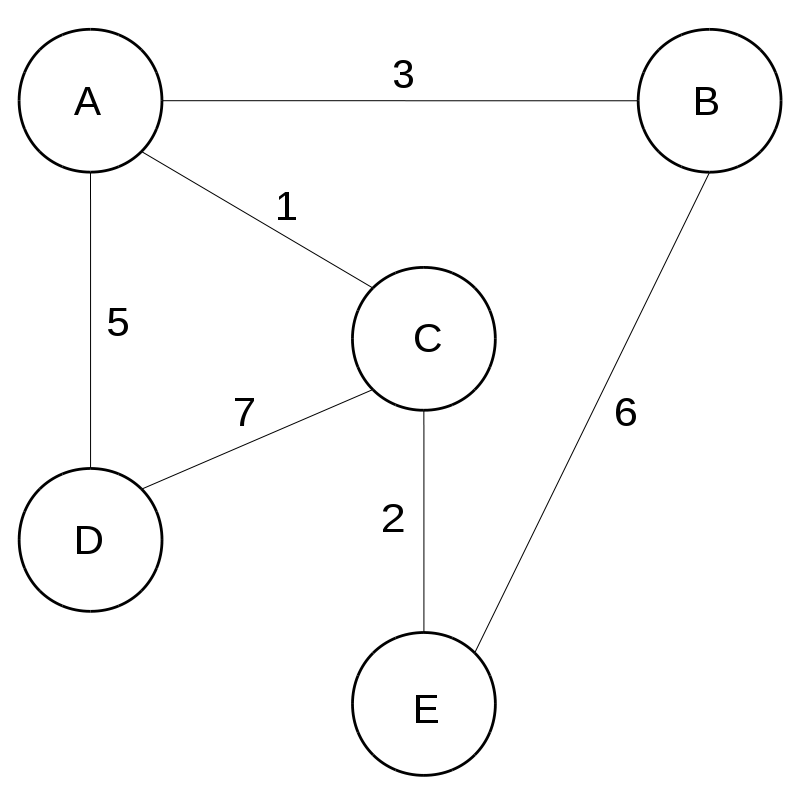
\includegraphics[width=12cm]{grafo.png}
\caption{Um grafo com 5 nós e 6 arestas.}
\label{fig:comun-intra-inter}
\end{figure}

%=====================================================
